% --- Template for thesis / report with tktltiki2 class ---
% 
% last updated 2013/02/15 for tkltiki2 v1.02

\documentclass[finnish]{tktltiki2}

% tktltiki2 automatically loads babel, so you can simply
% give the language parameter (e.g. finnish, swedish, english, british) as
% a parameter for the class: \documentclass[finnish]{tktltiki2}.
% The information on title and abstract is generated automatically depending on
% the language, see below if you need to change any of these manually.
% 
% Class options:
% - grading                 -- Print labels for grading information on the front page.
% - disablelastpagecounter  -- Disables the automatic generation of page number information
%                              in the abstract. See also \numberofpagesinformation{} command below.
%
% The class also respects the following options of article class:
%   10pt, 11pt, 12pt, final, draft, oneside, twoside,
%   openright, openany, onecolumn, twocolumn, leqno, fleqn
%
% The default font size is 11pt. The paper size used is A4, other sizes are not supported.
%
% rubber: module pdftex

% --- General packages ---

\usepackage[utf8]{inputenc}
\usepackage[T1]{fontenc}
\usepackage{lmodern}
\usepackage{microtype}
\usepackage{amsfonts,amsmath,amssymb,amsthm,booktabs,color,enumitem,graphicx}
\usepackage[pdftex,hidelinks]{hyperref}
\usepackage[ruled,vlined,linesnumbered]{algorithm2e}
\usepackage{caption}
\usepackage{float}
\usepackage{subcaption}
\usepackage{pdfpages}

% Algorithm2e environment with "Algoritmi"-caption.
\newenvironment{finalgo}[1][htb]{
  \renewcommand{\algorithmcfname}{Algoritmi}
  \begin{algorithm}[#1]
}{\end{algorithm}}

% To be able to not numbering individual lines:
\let\oldnl\nl% Store \nl in \oldnl
\newcommand{\nonl}{\renewcommand{\nl}{\let\nl\oldnl}}

% Automatically set the PDF metadata fields
\makeatletter
\AtBeginDocument{\hypersetup{pdftitle = {\@title}, pdfauthor = {\@author}}}
\makeatother

% --- Language-related settings ---
%
% these should be modified according to your language

% babelbib for non-english bibliography using bibtex
\usepackage[fixlanguage]{babelbib}
\selectbiblanguage{finnish}

% add bibliography to the table of contents
\usepackage[nottoc]{tocbibind}
% tocbibind renames the bibliography, use the following to change it back
\settocbibname{Lähteet}

% --- Theorem environment definitions ---

\newtheorem{lau}{Lause}
\newtheorem{lem}[lau]{Lemma}
\newtheorem{kor}[lau]{Korollaari}

\theoremstyle{definition}
\newtheorem{maar}[lau]{Määritelmä}
\newtheorem{ong}{Ongelma}
\newtheorem{alg}[lau]{Algoritmi}
\newtheorem{esim}[lau]{Esimerkki}

\theoremstyle{remark}
\newtheorem*{huom}{Huomautus}

\DeclareMathOperator*{\argmin}{arg\, min}

% --- tktltiki2 options ---
%
% The following commands define the information used to generate title and
% abstract pages. The following entries should be always specified:

\title{Polunhakualgoritmit ja -järjestelmät}
\author{Rodion Efremov}
\date{\today}
\level{Kandidaatintutkielma}
\abstract{Haettaessa lyhimpiä polkuja verkossa joudutaan väistämättä ottamaan kohdeverkon ominaisuuksia huomioon, mikäli tehtävästä halutaan suoriutua pienimmässä mahdollisessa ajassa. Toisinaan on mahdollista määritellä heuristiikkafunktio, ja siten käyttää A$^\ast$-perheen algoritmeja; toisinaan tätä ei voida tehdä, ei ainakaan tehokkaasti, jolloin jäljelle jää kaksisuuntaisuus ja/tai verkon esiprosessointi haun nopeuttamiseksi. Tämän tutkielman tarkoituksena on antaa (hyvin suppea) katsaus asiaan liittyviin algoritmeihin ja järjestelmiin.}

\keywords{verkot, lyhimmät polut}

% classification according to ACM Computing Classification System (http://www.acm.org/about/class/)
% This is probably mostly relevant for computer scientists
% uncomment the following; contents of \classification will be printed under the abstract with a title
% "ACM Computing Classification System (CCS):"
% \classification{}

% If the automatic page number counting is not working as desired in your case,
% uncomment the following to manually set the number of pages displayed in the abstract page:
%
% \numberofpagesinformation{16 sivua + 10 sivua liitteissä}
%
% If you are not a computer scientist, you will want to uncomment the following by hand and specify
% your department, faculty and subject by hand:
%
% \faculty{Matemaattis-luonnontieteellinen}
% \department{Tietojenkäsittelytieteen laitos}
% \subject{Tietojenkäsittelytiede}
%
% If you are not from the University of Helsinki, then you will most likely want to set these also:
%
% \university{Helsingin Yliopisto}
% \universitylong{HELSINGIN YLIOPISTO --- HELSINGFORS UNIVERSITET --- UNIVERSITY OF HELSINKI} % displayed on the top of the abstract page
% \city{Helsinki}
%


\begin{document}

% --- Front matter ---

\frontmatter      % roman page numbering for front matter

\maketitle        % title page
\makeabstract     % abstract page

\tableofcontents  % table of contents

% --- Main matter ---

\mainmatter       % clear page, start arabic page numbering

\section{Johdanto}
Polunhaku painotetuissa tai painottamattomissa verkoissa on perustavanlaatuinen ongelma, joka ei ole mielenkiintoinen vain itsessään, vaan myös tarvittavana alioperaationa muissa algoritmeissa. Esimerkiksi Edmond-Karpin algoritmi käyttää leveyssuuntaista hakua maksimivuo-ongelman ratkaisemiseksi \cite{Cormen09}. Viime vuosikymmeninä myös useamman sekvenssin rinnastusongelmaa on ruvettu ratkomaan heuristisin polunhakualgoritmein.

Verkko $G$ on pari $(V, A)$, jossa $V$ on solmujen joukko ja $A \subset V \times V$ on (suunnattujen) kaarien joukko. Suuntaamatonta verkkoa $G' = (V, E)$ voidaan aina simuloida suunnatulla verkolla $G= (V, A)$ siten, että jokaista suuntaamatonta kaarta $\{ u, v \} \in E$ kohti asetetaan $A$:han kaaret $(u, v)$ ja $(v, u)$. Suunnattu verkko on siis suuntaamattoman yleistys. Polunhakua varten verkosta erotellaan kaksi solmua: lähtösolmu $s$ ja maalisolmu $t$. Jatkossa, $n = |V|$ ja $m = |E|$; näin esimerkiksi leveyssuuntaisen haun aikavaativuus on $\mathcal{O}(n + m)$. Polku on $\gamma_k = \langle u_0, u_1, \dots, u_k \rangle$, missä mikään solmu ei esiinny yhtä kertaa enempää, ja verkossa on kaari $(u_i, u_{i + 1})$ jokaisella $i = 0, 1, \dots, k - 1$. Polkuun liittyvä kustannus on sen kaarien painojen summa. Painojen oletetaan olevan ei-negatiivisia. Painottamattomien verkkojen kohdalla jokaisen kaaren paino oletetaan olevan yksi.  Suunnatussa kaaressa $(u, v)$ $u$ kutsutaan $v$:n vanhemmaksi ja $v$ $u$:n lapseksi.

% --- References ---
%
% bibtex is used to generate the bibliography. The babplain style
% will generate numeric references (e.g. [1]) appropriate for theoretical
% computer science. If you need alphanumeric references (e.g [Tur90]), use
%
% \bibliographystyle{babalpha-lf}
%
% instead.
\section{Tavallisimmat algoritmit}
Keskusteltaessa polunhakualgoritmeista paras etenemissuunta lienee yleisimmistä tekniikoista ad-hoc ratkaisuihin. Optimaalin polun haku on intuitiivisinta painottamattomissa verkoissa, joissa niinkin helppo algoritmi kuin leveyssuuntainen haku (Algoritmi \ref{alg:bfs}) on riittävä. Algoritmi käyttää kahta tietorakennetta: saavutettujen solmujen FIFO-jonoa (engl. \textit{first-in, first-out}) ja hajautustaulua $\pi \colon V \to V \cup \{ \textbf{nil} \}$, joka assosioi jokaisen saavutetun solmun $u$ kanssa sen solmun $v$, josta haku on edennyt $u$:hun. Intuitio tämän takana on se, että leveyssuuntaisen haun hakuavaruus etenee yhden verkon tason kerrallaan lähtien lähtösolmusta $s$, kunnes se saavuttaa maalisolmun $t$, minkä jälkeen löydetty lyhin polku $\langle s = \pi(\pi(\dots)), \pi(\pi(t)), \pi(t), t \rangle$ voidaan rakentaa rutiinilla \textsc{Traceback-Path} (Algoritmi \ref{alg:tracepath}).
\begin{finalgo}
$u = x$ \\
$p = \langle  \rangle$ \\
\While{$u \textbf{\emph{ is not nil}}$}{
$p = \langle u \rangle \circ p$ \\
$u = \pi(u)$ \\
}
\nonl Kaksisuuntainen haku? \\
\If{$\pi_{REV} \textbf{\emph{ is not nil}}$}{
  $u = \pi_{REV}(x)$ \\
  \While{$u \textbf{\emph{ is not nil}}$}{
    $p = p \circ \langle u \rangle$ \\
    $u = \pi_{REV}(u)$ \\
  }
}
\KwRet $p$ \\
\caption{\textsc{Traceback-Path}$(x, \pi, \pi_{REV})$}
\label{alg:tracepath}
\end{finalgo}

\begin{finalgo}
  \SetKw{KwNil}{nil}
  \SetKw{KwIs}{is }
  \SetKw{KwNot}{not }
  \SetKw{KwMappedIn}{yet mapped in }
  $Q = \langle s \rangle$ \\
  $\pi(s) = \KwNil$ \\
  \While{$|Q| > 0$}{
    $u = \textsc{Dequeue}(Q)$ \\
    \If{$u $ \KwIs $t$}{
      \KwRet \textsc{Traceback-Path}$(u, \pi, \KwNil)$ \\
    }
    \For{$(u, v) \in G.A$}{
      \If{$v \; \KwIs \KwNot \KwMappedIn \pi$}{
        $\pi(v) = u$ \\
        $\textsc{Enqueue}(Q, v)$ \\
      }
    }
  }
  \KwRet $\langle \rangle$ \\
\caption{\textsc{Breadth-First-Search}$(G, s, t)$}
\label{alg:bfs}
\end{finalgo}

Mitä tulee painotettuihin verkkoihin, Edsger W. Dijkstra esitti vuonna 1959 kuuluisan polunhakualgoritminsa, joka toimii polynomisessa ajassa \cite{Dijkstra59}. Algoritmin voidaan katsoa yhdistävän ahneuden (engl. \textit{greedy algorithm}), dynaamisen ohjelmoinnin ja inkrementaalisen lähestymistavan. Saatuaan lähtösolmun $s$ algoritmi laskee lyhimpien polkujen puun lähtien solmusta $s$ kunnes solmu $t$ joutuu \textit{avoimeen listaan} (engl. \textit{open list; search frontier}), ja sitä kautta \textit{suljettuun listaan} (engl. \textit{closed list; settled node list}), jolloin lyhin $s, t$-polku on löytynyt. Hart et al. esittivät vuonna 1968 A$^{\ast}$-algoritminsa \cite{Hart68},  joka -- samoin kuten Djikstran algoritmi -- ylläpitää mm. kunkin saavutetun solmun $u$ $g$-arvon $g(u)$, joka on toistaiseksi pienin kustannus lähtösolmusta $s$ solmuun $u$, ja joka on taattu olemaan pienin mahdollinen heti kun $u$ poistuu avoimesta listasta. Erona on kuitenkin se, että A$^{\ast}$ käyttää kunkin solmun $u$ prioriteettinä sen $f$-arvoa, joka on $f(u) = g(u) + h(u)$, missä $h(u)$ on solmun $u$ optimistinen (eli aliarvioitu) etäisyys maalisolmuun. Heuristiikkafunktion optimistisuus on välttämätön, mikäli halutaan taata, että solmun $t$ poistuessa avoimesta listasta, vanhempifunktio $\pi$ antaa lyhimmän $s,t$-polun. Lisäksi, heuristiikkafunktio on \textit{monotoninen}, jos jokaisella kaarella $(u, v)$ on voimassa $h(u) \leq w(u, v) + h(v)$.
\begin{lau}
Jos heuristiikkafunktio $h \colon V \to \mathbb{R}$ on monotoninen, se on myös optimistinen (engl. \textit{admissible}).
\end{lau}
\begin{proof}
Olkoon solmut $v, t \in V$ annettu. Nyt $d(v, t)$ on lyhimmän polun $\langle v_0 = v, v_1, \dots, v_k = t \rangle$ kustannus 
\[
\sum_{i = 0}^{k - 1} w(v_i, v_{i + 1}).
\]
Heuristiikkafunktion monotonisuuden nojalla
\begin{align*}
h(v) &= h(v_0) \\
          &\leq w(v_0, v_1) + h(v_1) \\
          &\leq w(v_0, v_1) + w(v_1, v_2) + h(v_2) \\
          &\dots \\
          &\leq \sum_{i = 0}^{k - 1} w(v_i, v_{i + 1}) + h(v_k) \\
          &= d(v_0, v_k) + h(v_k) \\
          &= d(v, t) + h(t) \\
          &= d(v, t),
\end{align*}
sillä $h(t) = 0$.
\end{proof}
Intuitio tämän järjestelyn takana on se, että A$^{\ast}$ tietää mihin suuntaan haku on suunnattava, jota päästäisiin maalisolmuun, ainakin paremmin kuin Dijkstran algoritmi, jonka hakuavaruus kasvaa laajenevan pallon tavoin kaikkiin suuntiin. A$^{\ast}$:n pseudokoodi on tasan sama kuin Dijkstran algoritmin (Algoritmi \ref{alg:unidijkstra}). Erotuksena riveillä 14 ja 18 $g(x)$:n sijasta on $f(x)$, jolle siis $f(x) = g(x) + h(x)$. Molemmat kutsuvat \textsc{Traceback-Path}-rutiinia, joka muodostaa lyhimmän polun edeltäjäpuusta (engl. \textit{predecessor tree}) ajassa $\Theta(N)$, missä $N$ on lyhimmän polun solmujen määrä. On huomattava, että A$^{\ast}$ palautuu Dijkstran algoritmiin määrittelemällä $h(u) = 0$ jokaisella $u \in V$, sillä tuolloin $f(x) = g(x)$.
\begin{finalgo}
\nonl Monikkosijoitus \\
$\text{OPEN}, \text{CLOSED}, g, \pi = (\{ s \}, \emptyset, \{  (s, 0) \}, \{ (s, \textbf{nil}) \})$ \\
\While{$|\text{OPEN}| > 0$}{
 $u = \textsc{Extract-Minimum}(\text{OPEN})$ \\
 \If{$u \textbf{\emph{ is }} t$}{
   \KwRet \textsc{Traceback-Path$(u, \pi, \textbf{nil})$}\\
 }
 $\text{CLOSED} = \text{CLOSED} \cup \{ u \}$ \\
 \nonl Jokaisella solmun $u$ lapsisolmulla $x$, tee... \\
 \For{$(u, x) \in G.A$}{
   \If{$x \in \text{\upshape CLOSED}$}{
     $\textbf{continue}$ \\
   }
   $g' = g(u) + w(u, x)$ \\
   \If{$x \not \in \text{\upshape OPEN}$}{
     $g(x) = g'$ \\
     $\pi(x) = u$ \\
     $\textsc{Insert}(\text{OPEN}, x, g(x))$ \\
   }
   \ElseIf{$g(x) > g'$}{
     $g(x) = g'$ \\
     $\pi(x) = u$ \\
     $\textsc{Decrease-Key}(\text{OPEN}, x, g(x))$ \\
   }
 }
}
\nonl Ei $s, t$ -polkua verkossa $G$. \\
\KwRet $\langle \rangle$ \\
\caption{\textsc{Dijkstra-Shortest-Path}$(G, s, t, w)$}
\label{alg:unidijkstra}
\label{Dijkstra}
\end{finalgo}

\subsection{Prioriteettijonon valinta}
Polkua haettaessa painotetussa verkossa joudutaan käyttäämään prioriteettijonoja, jotka ovat tarpeellisia hakujen pitämiseksi optimaalisina, ja joiden oletetaan tarjoavan ainakin seuraavat operaatiot:
\begin{enumerate}
\item \textsc{Insert}$(H, x, k)$ tallettaa solmun $x$ sen prioriteettiavaimen $k$ kera,
\item \textsc{Decrease-Key}$(H, x, k)$ päivittää solmun $x$ talletetun prioriteettiavaimen (pienemmäksi),
\item \textsc{Extract-Minimum}$(H)$ poistaa pienimmän prioriteetin omaavan solmun, 
\item \textsc{Min}$(H)$ palauttaa, muttei poista keosta solmua, jolla on pienin prioriteettiavain, ja
\item $|H|$ palauttaa jonossa olevien alkioiden määrän.
\end{enumerate}
Operaatiot (4) ja (5) voidaan aina toteuttaa siten, että ne toimivat vakioajassa. Helpoin prioriteettijonorakenne (jatkossa vain \textit{keko}), jonka operaatiot (1) - (3) käyvät logaritmisessa ajassa, on binäärikeko. Tällaisella keolla Dijkstran ja A$^{\ast}$-algoritmit käyvät kumpikin ajassa $\mathcal{O}((m + n) \log n)$. Teoriassa edelläolevaa yllärajaa voidaan parantaa käyttämällä Fibonacci-kekoa, jonka lisäysoperaatio (1) toimii eksaktissa vakioajassa, päivitysoperaatio (2) tasoitetussa vakioajassa, ja poisto-operaatio (3) tasoitetussa ajassa $\mathcal{O}(\log n)$. Tällöin haut voidaan suorittaa ajassa $\mathcal{O}(m + n \log n)$. Huomaa, että kaikki tähän asti mainitut keot perustuvat vertailuihin, ja teoriassa enintään yksi operaatiosta \textsc{Insert} tai \textsc{Extract-Minimum} voi käydä eksaktissa tai tasoitetussa vakioajassa, ja toisen on käyttävä ajassa $\Omega(\log n)$, koska muuten algoritmi \ref{alg:genheapsort} tällaisella keolla rikkoisi vertailuihin perustuvan lajittelemisen informaatioteoreettisen rajan, joka on $\Omega(n \log n)$. 

\begin{finalgo}[p]
\nonl \text{Tyhjennä keko} \\
$H = \varnothing$ \\
\For{i = 1 \emph{\KwTo} |S|}{
  \nonl $S[i]$ on itsensä prioriteetti. \\
  \textsc{Insert}$(H, S[i], S[i])$ \\
}
\For{i = 1 \emph{\KwTo} |S|}{
  $S[i] = $\textsc{Extract-Minimum}$(H)$  \\
}
\caption{\textsc{Generic-Heap-Sort}($S, H$)}
\label{alg:genheapsort}
\end{finalgo}

Jos kuitenkin kaarien painot ovat kokonaislukuja, $\mathcal{O}(m + n \log n)$-rajaa voidaan parantaa:
Mikkel Thorup esitti vuonna 2003 keon, jonka poisto-operaatio toimii ajassa $\mathcal{O}(\log \log \min n)$ ja muut operaatiot vakioajassa \cite{Thorup03}. Jos kuitenkin kokonaislukupainot ovat väliltä $[0, N)$, poisto-operaatio voidaan suorittaa ajassa $\mathcal{O}(\log \log \min \{ n, N \})$. Nyt selvästi haun aikavaativuus tällaisella keolla on $\mathcal{O}(m + n \log \log \min \{n, N \})$. Lisäksi Dial on esittänyt liki triviaalin prioriteettijonon, joka soveltuu erityisesti kokonaislukuprioriteettiavaimiin väliltä $[0, U]$, missä $U$ ei ole suuri (esimerkiksi alle 200), ja jonka lisäys- ja päivitysoperaatiot toimivat vakioajassa ja poisto-operaatio ajassa $\mathcal{O}(U)$, jolloin tällainen rakenne voi olla toivottava heuristisessa painottamattomassa haussa, kuten esimerkiksi $(n^2 - 1)$-palapelissä (engl. \textit{8-puzzle, 15-puzzle, ...}).

\section{Kaksisuuntainen haku}
Vaikka A$^{\ast}$ on tyypillisesti tehokkaampi kuin Dijkstran algoritmi, käyttämällä \textit{kaksisuuntaista} hakua, voidaan päästää verrattavissa olevaan suorituskykyyn. Ajatus kaksisuuntaisuuden takana on se, että algoritmi kasvattaa kaksi hakupuuta: yhden normaaliin tapaan ja toisen maalisolmusta ihan kuin kaaret olisi käännetty päinvastaiseen suuntaan, kunnes kaksi hakuavaruutta kohtaavat keskellä. Nyt jos lyhin polku koostuu $N$ kaaresta, ja verkon solmujen keskiarvoinen aste on $d$, tavallinen eli yksisuuntainen haku vaatii ajan
\[
\sum_{i = 0}^N d^i,
\]
kun kaksisuuntainen vaatii
\[
2 \sum_{i = 0}^{\lceil N / 2 \rceil} d^i.
\]
Ylläoleva pätee leveyssuuntaiseen hakuun sellaisenaan, ja painotetun haun kohdalla voidaan saada yläraja kertomalla kunkin summan termi tekijällä $\mathcal{O}(\log n)$, joka liittyy algoritmien käyttämän prioritettijonon operaatioihin. 

\subsection{Kaksisuuntainen leveyssuuntainen haku}
Leveyssuuntainen haku hyötyy kaksisuuntaisuudesta, vaikka toteutus vaatii kuusi erilaista tietorakennetta: kaksi FIFO-jonoa $Q$ ja $Q_{REV}$ (kumpikin on riittävä mallintamaan prioriteettijonoja painottomassa haussa). Lisäksi tarvitaan edeltäjäkuvaukset kumpaakin hakusuuntaa varten: $\pi$ ja $\pi_{REV}$. Etäisyyskuvauksien $d$ ja $d_{REV}$ rooli on analoginen Dijkstran algoritmin $g$-kuvauksen kanssa: $d(u)$ on lyhimmän $s, u$-polun kaarien määrä (ja siten myös kustannus) ja $d_{REV}(u)$ on lyhimmän $u, t$-polun kustannus. Aina kun tietyssä hakusuunnassa poistetaan jonosta solmu $x$, tarkistetaan joko vastakkaisen hakusuunnan kuvauksissa on kuvaus solmulle $x$. Jos asia on niin, on löydetty välisolmu, johon molemmat hakusuunnat ovat edenneet, ja jos edellä mainittu $x$, jonka implikoima polun kustannus on $d(x) + d_{REV}(x)$, parantaa toistaiseksi parhaan tunnetun polun kustannuksen $\mu$, $x$ talletetaan välisolmuksi $m$, josta myöhemmin rutiini \textsc{Traceback-Path} (Algoritmi \ref{alg:tracepath}) pystyy muodostomaan lyhimmän polun. Yksi mahdollinen rajoite kaksisuuntaisen haun käyttöönotolle on se, että jos painottamattomassa verkossa on useampi lyhin polku, kaksisuuntainen versio ei välttämättä löydä samaa polkua kuin tavallinen. Tämä saattaa olla joissakin sovelluksissa ongelmallista mikäli on tarvetta laajentaa kunkin jonosta poistetun solmun seuraajasolmut tietyssä järjestyksessä.
\begin{finalgo}[p]
  \SetKw{KwNil}{nil}
  \SetKw{KwIs}{is }
  \SetKw{KwNot}{not }
  \SetKw{KwYetMappedIn}{yet mapped in }
  \SetKw{KwMappedIn}{mapped in }
  \SetKw{KwAnd}{and }
  $Q, \pi, d = (\langle s \rangle, (s, \KwNil), (s, 0))$ \\
  $Q_{REV}, \pi_{REV}, d_{REV} = (\langle t \rangle, (t, \KwNil), (t, 0))$ \\
  $m, \mu = (\KwNil, \infty)$ \\
  \While{$|Q| > 0$ \KwAnd $|Q_{REV}| > 0$}{
    \If{$m$ \KwIs \KwNot \KwNil \KwAnd $d(\textsc{Head}(Q)) + d_{REV}(\textsc{Head}(Q_{REV})) \geq \mu$}{
        \KwRet \textsc{Traceback-Path}$(m, \pi, \pi_{REV})$ \\
    }
    $u = \textsc{Dequeue}(Q)$ \\
    \If{$u$ \KwIs \KwMappedIn $\pi_{REV}$ \KwAnd $\mu > d(u) + d_{REV}(u)$}{
        $\mu = d(u) + d_{REV}(u)$\\
        $m = u$ \\
    }
    \For{$(u, v) \in G.A$}{
      \If{$v \; \KwIs \KwNot \KwYetMappedIn \pi$}{
        $\pi(v) = u$ \\
        $d(v) = d(u) + 1$ \\
        $\textsc{Enqueue}(Q, v)$ \\
      }
    }
    $u = \textsc{Dequeue}(Q_{REV})$ \\
    \If{$u$ \KwIs \KwMappedIn $\pi$ \KwAnd $\mu > d(u) + d_{REV}(u)$}{
        $\mu = d(u) + d_{REV}(u)$\\
        $m = u$ \\
    }
    \For{$(v, u) \in G.A$}{
      \If{$v \; \KwIs \KwNot \KwYetMappedIn \pi_{REV}$}{
        $\pi_{REV}(v) = u$ \\
        $d_{REV}(v) = d_{REV}(u) + 1$ \\
        $\textsc{Enqueue}(Q_{REV}, v)$ \\
      }
    }
  }
  \KwRet $\langle \rangle$ \\
\caption{\textsc{Bidirectional-Breadth-First-Search}$(G, s, t)$}
\end{finalgo}

\subsection{Kaksisuuntainen Dijkstran algoritmi}
Ylläolevan analyysin nojalla on selvää, että Dijkstran algoritmi hyötyy kaksisuuntaisuudesta eikä edellytä minkäänlaista verkon esiprosessointia. Lisäksi algoritmin vahvuutena suhteessa A$^{\ast}$:iin ei ole pelkästään verrattavissa oleva tehokkuus, vaan myös heuristiikkafunktion tarpeettomuus. Toistaiseksi lyhimmän polun kustannus pidetään muuttujassa $\mu$, jonka arvoksi suorituksen alussa asetetaan $\infty$. Kun algoritmi löytää toistaiseksi lyhimmän polun hakuavaruuksien kohdatessa, välisolmu $m$ ja sen implikoima kustannus $\mu$ päivitetään. Haku jatkuu siihen asti, kunnes molempien avointen listojen minimialkioiden kustannusten summa on vähintään $\mu$. 

Molemmat hakusuunnat käyttävät alirutiinia \textsc{Expand}, mutta eri parametrein: listat OPEN ja CLOSED kuuluvat saman suunnan dataan (suunta $d$), $\text{CLOSED}_2$ on vastakkaisen hakusuunnan $\hat{d}$ suljettu lista, $g, \pi$ ovat suunnan $d$ kustannuskuvaus ja vanhempainkuvaus vataavasti, $m$ on toistaiseksi lyhimmän polun välisolmu, jossa kaksi hakuavaruutta kohtaavat, $\mu$ on $m$:n implikoiman polun kustannus, $\ast$ on laajentumisoperaattori, jolle $\ast(u)$ antaa solmun $u$ seuraajasolmut, ja kuvaus $w \colon A \to \mathbb{R}_{\geq 0}$ antaa kaarien painot. Yllä suunta $d$ ei ole vakio, vaan suuntaa merkitseva muuttuja, jolle $\hat{d}$ on vastakkainen suunta. Parametrit otaksutaan tässä rutiinissa viiteparametreiksi, jolloin esimerkiksi $\mu$ ja $m$ ovat päivitettävissä. 

Rutiini \textsc{Update} tarkistaa, että yhden hakusuunnan solmu on toisen suljetussa listassa, ja jos asia on niin, yrittää päivittää välisolmun ja siihen liittyvän toistaiseksi pienimmän kustannuksen $\mu$ ja se vaatii parametreikseen hakusuunnan $d$ solmun $x$, suunnan $\hat{d}$ CLOSED-listan, solmun $x$ $g$-arvo $g_x$ suunnassa $d$, suunnan $\hat{d}$ $g$-kuvauksen, välisolmun $m$ ja sen implikoiman kustannuksen $\mu$. Tämänkin apurutiinin kohdalla parametrit otaksutaan viiteparametreiksi, jolloin niiden päivittäminen rutiinissa on mahdollista.

Laajentumisoperaattoreina (engl. \textit{expansion operator}) kaksisuuntaisessa haussa on määriteltävä funktiot $e, e_{REV} \colon V \to \mathcal{P}(V)$, joille $e(u) = \{ v \in V \colon (u, v) \in A \}$ ja $e_{REV}(u) = \{ v \in V \colon (v, u) \in A \}$. Nyt siis $e(u)$ antaa solmun $u$ lapsisolmut, ja $e_{REV}(u)$ sen vanhempisolmut, jolloin $e$:tä käytetään normaalissa ja $e_{REV}$:tä käännetyssä haussa. Rutiini \ref{alg:bidijkstraterminate} määrittelee kaksisuuntaisen Dijkstran algoritmin pysähtymisehdon, joka on tarpeeksi vahva pitämään polut optimaaleina ja laskenta-ajan kohtuullisena.
\begin{finalgo}[p]
\SetKw{KwIs}{is}
$u = \textsc{Extract-Minimum}(\text{OPEN})$ \\
\text{CLOSED} = \text{CLOSED} $\cup \, \{ u \}$ \\
\For{$x \in \ast(u)$}{
  \If{$x \in \text{CLOSED}$}{
    \textbf{continue} \\
  }
  $g' = g(u)$ \\
  \If{$\ast$ \KwIs $e_{REV}$}{
    \nonl Käännetty haku. \\
    $g' = g' + w(x, u)$ \\
  }
  \Else {
    \nonl Normaali haku. \\
    $g' = g' + w(u, x)$ \\
  }
  \If{$x \not \in \text{OPEN}$}{
    $g(x) = g'$ \\
    $\pi(x) = u$ \\
    \textsc{Insert}$(\text{OPEN}, x, g(x))$ \\
    \textsc{Update}$(x, \text{CLOSED}_2, g(x), g_2, \mu, m)$ \\
  }
  \ElseIf{$g(x) > g'$}{
    $g(x) = g'$ \\
    $\pi(x) = u$ \\
    \textsc{Decrease-Key}$(\text{OPEN}, x, g(x))$ \\
    \textsc{Update}$(x, \text{CLOSED}_2, g(x), g_2, \mu, m)$ \\
  }
}
\caption{\textsc{Expand}$(\text{OPEN, CLOSED, CLOSED}_2, g, g_2, \pi, \mu, m, \ast, w)$}
\label{alg:expand}
\end{finalgo}
\begin{finalgo}[p]
\If{$x \in \text{CLOSED}$}{
   $p = g_x + g(x)$ \\
   \If{$\mu > p$}{
     $\mu = p$ \\
     $m = x$ \\
   }
}
\caption{\textsc{Update}$(x, \text{CLOSED}, g_x, g, \mu, m)$}
\label{alg:update}
\end{finalgo}
\begin{finalgo}[p]
\If{$g(\textsc{Min(OPEN)}) + g_{REV}(\textsc{Min}(\textsc{OPEN}_{REV})) \geq \mu$}{
  \KwRet \textsc{Traceback-Path}$(m, \pi, \pi_{REV})$\\
}
\KwRet $\textbf{nil}$ \\
\caption{\textsc{Terminate}$(\text{OPEN}, \text{OPEN}_{REV}, g, g_{REV}, \pi, \pi_{REV}, \mu, m)$}
\label{alg:bidijkstraterminate}
\end{finalgo}

\begin{finalgo}[p]  
\SetKw{KwAnd}{and}
$\text{OPEN}, \text{CLOSED}, g, \pi = \{ s \}, \emptyset, \{ (s, 0) \}, \{ (s, \textbf{nil}) \}$ \\
$\text{OPEN}_{REV}, \text{CLOSED}_{REV}, g_{REV}, \pi_{REV} = \{ t \}, \emptyset, \{ (t, 0) \}, \{ (t, \textbf{nil}) \}$ \\
$\mu = \infty$ \\
$m = \textbf{nil}$ \\ 
\While{$|\textsc{OPEN}| > 0$ \KwAnd $|\textsc{OPEN}_{REV}| > 0$}{
  \If{$m$ \textbf{\emph{is not nil}}}{
    $p = \textsc{Terminate}(\text{OPEN}, \text{OPEN}_{REV},$ \\
    $\phantom{p = \textsc{Terminate}(} g, g_{REV},$ \\
    $\phantom{p = \textsc{Terminate}(} \pi, \pi_{REV},$  \\
    $\phantom{p = \textsc{Terminate}(} \mu, m)$ \\
    \If{$p$ \textbf{\emph{is not nil}}}{
    	\KwRet $p$
    }
  }
  \nonl Triviaali kuormantasaus \\
  \If{$|\textsc{OPEN}| < |\textsc{OPEN}_{REV}|$}{
	$\textsc{Expand}(\text{OPEN},$ \\
	$\phantom{\textsc{Expand}(}\text{CLOSED},$ \\
	$\phantom{\textsc{Expand}(}\textsc{CLOSED}_{REV},$ \\ 
	$\phantom{\textsc{Expand}(}g, g_{REV}, \pi, \mu, m, e, w)$ \\
  }
  \Else{
	$\textsc{Expand}(\text{OPEN}_{REV},$ \\
	$\phantom{\textsc{Expand}(}\text{CLOSED}_{REV},$ \\
	$\phantom{\textsc{Expand}(}\textsc{CLOSED},$ \\ 
	$\phantom{\textsc{Expand}(}g_{REV}, g, \pi_{REV}, \mu, m, e_{REV}, w)$ \\
  }
}
\KwRet $\langle  \rangle$ \\
\caption{\textsc{Bidirectional-Dijkstra-Shortest-Path}$(G, s, t, w)$}
\label{alg:bidijkstra}
\end{finalgo}

\subsection{Kaksisuuntainen A$^{\ast}$}
Kaksisuuntaisen A$^{\ast}$:n saa aikaan muuttamalla algoritmin \textsc{Expand} (Algoritmi \ref{alg:expand}) riveillä 14 ja 19  esiintyvät $g(x)$ $f(x)$:ksi ja muuttamalla \textsc{Terminate}-rutiinin ehdon seuraavanlaiseksi:
\[
\max (f(\textsc{Min}(\text{OPEN})), f_{REV}(\textsc{Min}(\text{OPEN}_{REV}))) \geq \mu,
\]
joka on Ira Pohlin vuonna 1971 ehdottaman BHPA-algoritmin pysähtymisehto \cite{Pohl71}.
Yllä $f_{REV}(u) = g_{REV}(u) + h_{REV}(u)$, missä $h_{REV}(u)$ antaa optimistisen arvion solmun $u$ etäisyydestä lähtösolmusta $s$.

Vuonna 2007 Taeg-Keun Whangbo ehdotti toisenlaisen kaksisuuntaisen heuristisen hakualgoritmin \cite{Whangbo07}, joka olettaa, että kullakin solmulla $u$ on koordinaatit tasossa $c(u) = (u_1, u_2) \in \mathbb{R}^2$. $h$-arvon sijasta, määritellään
\begin{align*}
l(x) &= \frac{[c(s) - c(p)] \cdot [c(x) - c(p)]}{ | c(s) - c(p) | }, x \in \text{OPEN}, \\
l_{REV}(x) &= \frac{[c(t) - c(p)] \cdot [c(x) - c(p)]}{ | c(t) - c(p) | }, x \in \text{OPEN}_{REV}.
\end{align*}

Kun kaksi hakuavaruutta kohtaavat solmussa $p$, piirretään $p$:n kautta kulkeva suora $\Lambda$, joka on normaali sen suoran kanssa, joka kulkee solmujen $s, t$ kautta. Nyt esimerkiksi jokaisella $x \in \text{OPEN}$, $l(c(x))$ on solmun $x$ etäisyys $\Lambda$:sta,
\begin{figure}
  \centering
  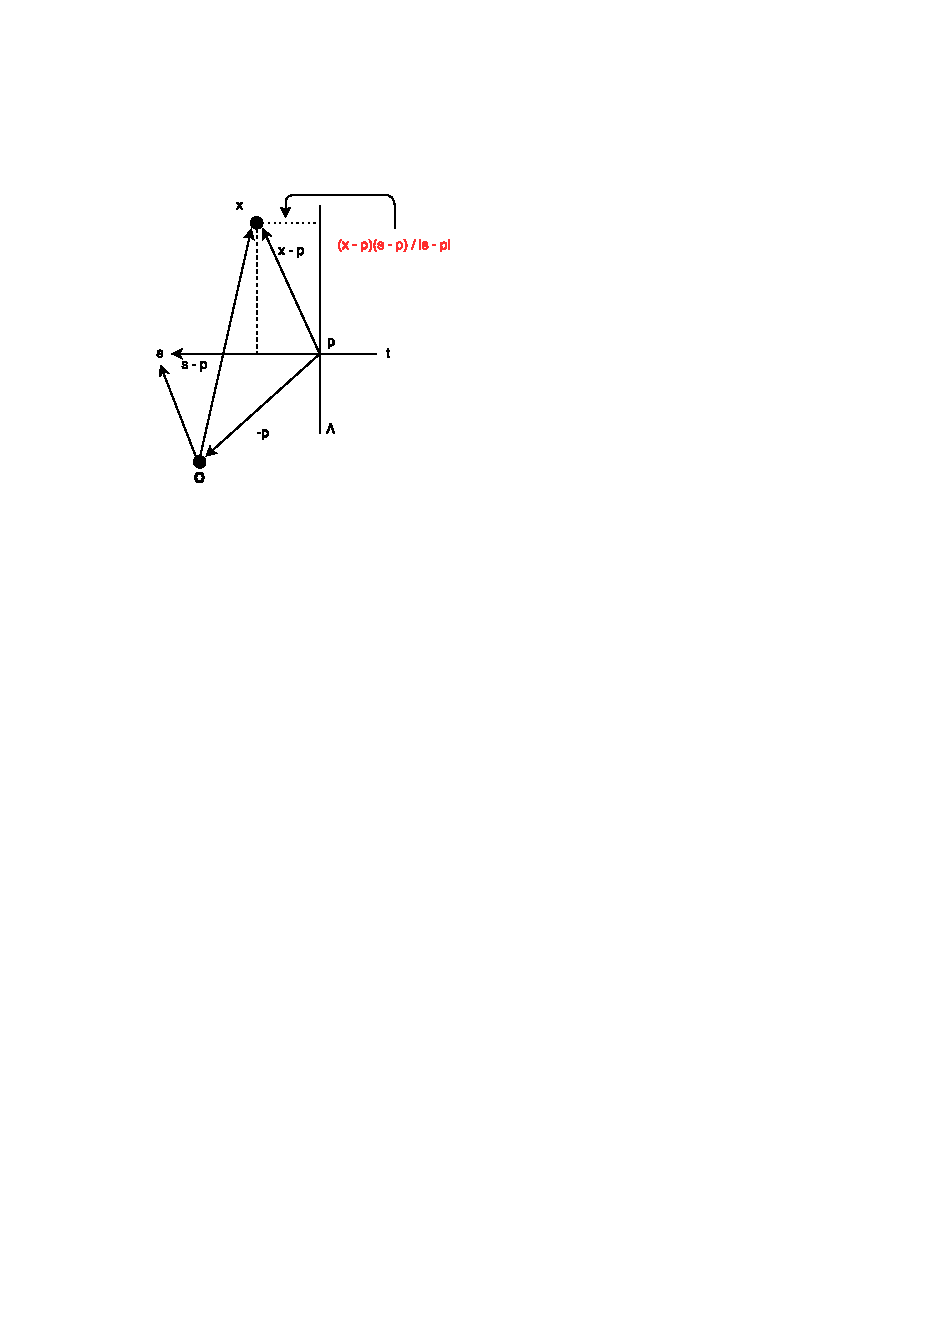
\includegraphics[trim=-1cm 15cm 0cm 4cm,width=550px,keepaspectratio]{Whangbo.pdf}
  \label{fig:whangbo}
  \caption{$l(c(x))$}
\end{figure}
kuten kuvasta 1 ilmenee, ja uusi pysähtymisehto on
\begin{align*}
L^1_{\min} & \leq \underset{x \in \text{OPEN}}{\min} (g(x) + l(x)), \\
L^2_{\min} & \leq \underset{x \in \text{OPEN}_{REV}}{\min} (g_{REV}(x) + l_{REV}(x)),
\end{align*}
missä $L_{\min}^1$ on lyhimmän $s, p$ -polun kustannus normaalin haun puussa, ja $L_{\min}^2$ analogisesti lyhimmän $p, t$ -polun kustannus vastakkaissuuntaisessa haussa. Kun algoritmin toiminta päättyy, lyhimmän polun kustannus on $L^1_{\min} + L^2_{\min}$. Whangbo raportoi tavallisen A$^{\ast}$:n vievän yhteensä 372 aikayksikköä laskettuna yhteen yli joukon hakuja. Samalla datalla BHPA vie 509 aikayksikköä, ja Whangbon variantti 209 aikayksikköä (huomaa BHPA:n vievän enemmän aikaa kuin tavallinen A$^{\ast}$).

\section{Kaikkien parien lyhimmät polut}
Toisinaan on annettu $n$ solmua ja halutaan löytää lyhimmät polut kaikkien solmuparien välillä. Yksi tehokkaimmista algoritmeista on Floyd-Warshallin algoritmi, joka toimii ajassa $\Theta(n^3)$, eikä sen toiminta riipu kaarien määrästä $m$. Ellei kohdeverkko ole täysi ($m = o(n^2)$), Johnsonin algoritmi saattaa olla parempi valinta, sillä Fibonacci-keolla edellämainittu käy ajassa $\mathcal{O}(n^2 \log n + nm)$. 

\subsection{Floyd-Warshall -algoritmi}
Vaikka Floyd-Warshall -algoritmin aikavaativuus ei ole koskaan Johnsonin algoritmin aikavaativuutta parempi, käytännössä Floyd-Warshall saattaa olla tehokkaampi vaihtoehto, sillä sen toteutus on vain kolme sisäkkäistä silmukkaa, joista kukin iteroidaan $n$ kertaa, ja sisimmän silmukan rungossa tehdään vain yksinkertainen testi, jolloin koko algoritmin aikavaativuuteen liittyvät vakiokertoimet ovat pieniä. Polunmuodostusrutiini \textsc{Build-Path} (Algoritmi \ref{alg:buildpath}) eroaa yllä esitetystä rutiinista \textsc{Traceback-Path} (Algoritmi \ref{alg:tracepath}). Yllä on oletettu, että kokonaisluvut $1, 2, \dots, n$ esittävät solmujoukon: tällöin voidaan aina johtaa bijektio $\{ 1, 2, \dots, n \} \to V_{domain}$, jolla kuvataan yhden esitystavan solmut toisen esitystavan solmuihin.
\begin{finalgo}[h]
  \SetKw{KwNil}{nil}
  $d = \mathbb{R}^{n \times n}$ \\
  $\pi = \mathbb{N}^{n \times n}$ \\
   \For{$i = 1$ \KwTo $n$}{
     \For{$j = 1$ \KwTo $n$}{
       $d(i, j) = w(i, j)$ \\
       \If{$w(i, j) \neq \infty$}{
         $\pi(i, j) = j$ \\
       }
       \Else{
         $\pi(i, j) = $ \KwNil \\
       }
     }
   }
   \For{$k = 1$ \KwTo $n$}{
     \For{$i = 1$ \KwTo $n$}{
       \For{$j = 1$ \KwTo $n$}{
         \If{$d(i, j) > d(i, k) + d(k, j)$}{
           $d(i, j) = d(i, k) + d(k, j)$ \\
           $\pi(i, j) = \pi(i, k)$ \\
         }
       }
     }
   }
   \KwRet $(d, \pi)$ \\
\caption{\textsc{Floyd-Warshall}$(n, w)$}
\label{alg:warshall}
\end{finalgo}

Intuitio Floyd-Warshallin algoritmin takana on se, että se tutkii, voidaanko parantaa nykyisen $i, j$-polun kustannus menemällä solmun $k$ kautta ja jos voidaan, molemmat matriisit päivitetään kuvastamaan sitä tilannetta, ja koska Floyd-Warshall iteroi kaikkien kolmikkoiden $(k, i, j) \in \{ 1, 2, \dots, n \}^3$
yli, se ratkaisee kaikkien-parien lyhimmät polut optimaalisesti.

\subsection{Johnsonin algoritmi}
Johnsonin algoritmi lisää syöteverkon solmujoukkoon uuden solmun $q$, kaaret $(q, v)$ kaikilla $v \in V$, ja asettaa kunkin edellä mainitun kaaren painoksi 0. Sen jälkeen algoritmi ajaa Bellman-Ford -algoritmin solmusta $q$ lähtien: jos on löytynyt negatiivisen painon omaava sykli, Johnsonin algoritmin toiminta päättyy. 
Negatiivisen painon omaava sykli on jono $\langle v_1, v_2, \dots, v_k \rangle$, missä $v_1 = v_k$, muut solmut kuin $v_1 = v_k$ esiintyvät vain kerran ja 
\[
\sum_{i = 1}^{k - 1} w(v_i, v_{i +1}) + w(v_k, v_1) < 0.
\]
Mikäli verkossa ei ole negatiivisia sykleja, rakennetaan jokaisesta solmusta lähtien kokonaiset lyhimpien polkujen puut ja sen mukaan kun jokainen puu valmistuu, poimitaan siitä asianomaisten polkujen painot ja talletetaan ne kustannus- ja edeltäjämatriiseihin. Koska Dijkstran algoritmi olettaa kunkin kaaren painon ei-negatiiviseksi, jos verkossa on sellaisia, Johnsonin algoritmi joutuu käyttämään toisenlaista painofunktiota $\hat{w}(u, v) = w(u, v) + h(u) - h(v)$ (uudelleenpainotus), missä $h(u) = \delta(q, u)$, joka on Bellman-Fordin tuottama lyhin $q, u$-kustannus.

\subsection{Soveltuvuus}
Yllä esitetyistä aikavaativuuksista ilmenee, etteivät asianomaiset algoritmit ole tarpeeksi tehokkaita ainakaan $n$:n arvoilla $\geq$ 10000. Jos kuitenkin ongelman koko sallii kaikkien parien algoritmin ajon, algoritmi palauttaa edeltäjämatriisin (engl. \textit{predecessor matrix}), josta $N$:n solmun lyhin polku voidaan rakentaa ajassa $\Theta(N)$, mitä ei pysty parantamaan tuon enempää, ei ainakaan ilman edistynempää algoritmiikkaa. (Ja vaikka voisikin, polun tulostaminen ja/tai piirtäminen on jo vähintään $\Omega(N)$.)
\begin{finalgo}[t]
\SetKw{KwNil}{nil}
\If{$\pi(i, j) = $ \KwNil}{
  \KwRet $\langle \rangle$ \\
}
$p = \langle i \rangle$ \\
\While{$i \neq j$}{
  $i = \pi(i, j)$\\
  $p = p \circ \langle i \rangle $\\
}
\KwRet $p$ \\
\label{alg:buildpath}
\caption{\textsc{Build-Path}$(\pi, i, j)$}
\end{finalgo}

\section{Ruudukkoverkko ja jump point -haku}
Ruudukkoverkko (engl. \textit{grid graph}) on suuntaamattoman verkon erikoistapaus, ja sen rakenne voidaan määritellä siten, että kullakin solmulla on kahden kokonaisluvun koordinaatti, eli solmujoukko on $\{ (x, y) \colon 1 \leq x \leq w, 1 \leq y \leq h \}$, missä $w$ on ruudukkoverkon leveys ja $h$ on sen korkeus. Nyt kun on annettu kaksi solmua $(x_1, y_1)$ ja $(x_2, y_2)$, jos vain yksi koordinaateista eroaa yksikön verran, kyseessä on vaaka- tai pystysuuntainen kaari ja sen painoksi asetetaan 1. Toisaalta, kun molemmat koordinaatit eroavat yksikön verran, kyseessä on vino kaari, jonka painoksi asetetaan $\sqrt{2}$. On selvää, että jo leveyssuuntainen haku on optimaali tällaisella verkolla, sillä aina kun se etenee vinottain, esim. solmusta $(x, y)$ solmuun $(x + 1, y - 1)$, se ohittaa kahden kaaren siirron solmun $(x + 1, y)$ tai $(x, y - 1)$ kautta, joka pidentäisi lyhimmän polun pituuden kahdella yksiköllä $\sqrt{2}$ sijaan. Heuristinen haku on kannattavaa tällaisella verkkotyypillä, sillä heuristiset funktiot kuten euklidinen (tai Manhattan-metriikka, ellei vinoja kaareja sallita) on helppo toteuttaa ilman esiprosessointia. Toisaalta, juuri tällaisella verkkotyypillä $A\ast$ kärsii polkujen ''symmetriasta'', kuten kuvasta \ref{fig:astarpathsymmetry} ilmenee. Jos siis solmujen $s$ ja $t$ molemmat koordinaatit eroavat, $A\ast$ kasvattaa suunnikkaanmuotoisen hakuavaruuden solmusta $s$ solmuun $t$, sillä niiden välissä on monta saman kustannuksen omaavaa polkua. Kuten yleensä erikoistapauksiin  rajoituttaessa, polunhaku ruudukolla voidaan tehdä paljon tehokkaammin. Vuonna 2011 Harabor ja Grastien esittivät ''jump point search'' -nimisen $A\ast$:n muunnelman, joka karsii pois polkusymmetriat ja etenee ''hyppien'' yli monen solmun siinä, missä muut algoritmit etenevät jokaisen välisolmun kautta \cite{Harabor11}.
\begin{figure}
  \centering
  \begin{subfigure}[h]{0.45\textwidth}
    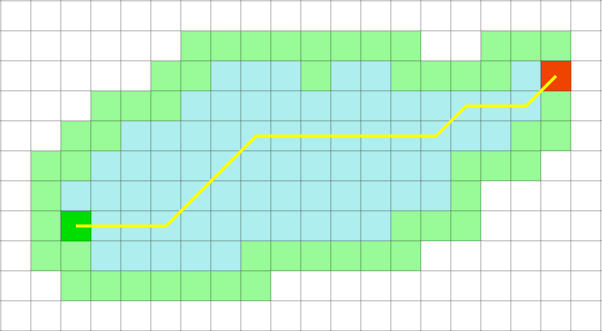
\includegraphics[clip=true,trim = 8px 8px 8px 8px,width=\textwidth,keepaspectratio]{AStarSearch}
    \caption{A$^{\ast}$-haku}
    \label{fig:astarpathsymmetry}
  \end{subfigure}
  ~
  \begin{subfigure}[h]{0.45\textwidth}
    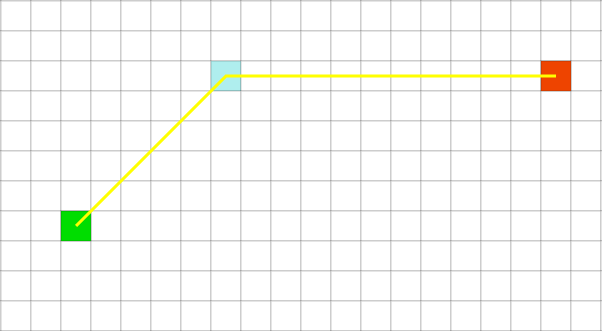
\includegraphics[clip=true,trim = 8px 8px 8px 8px,width=\textwidth,keepaspectratio]{JumpPointSearch}
    \caption{Jump point -haku}
  \end{subfigure}
  \caption{Polkusymmetria}
\end{figure}

\section{Dijkstran algoritmi kaarivivuilla}
Vuonna 2007 Möhring et al. esittivät mielenkiintoisen tavan nopeuttaa Dijkstran algoritmia \cite{Mohring07}. Ajatuksena on osittaa suunnatun verkon $G=(V, A)$ solmujoukko osioihin $V_1, \dots, V_p$ siten, että
\[
\bigcup_{i = 1}^p V_i = V,
\]
ja $V_i \cap V_j = \emptyset$ jokaisella $i \neq j$. Ositus voidaan toteuttaa kuvauksella $r \colon V \to \{1, \dots, p\}$. Kustakin osiosta $V_i$ puhuttaessa, sen ''rajasolmut'' (engl. \textit{boundary nodes}) määritellään joukkona
\[
B_i = \{ v \in V_i \colon \exists(u, v) \in A \text{ siten että } r(v) \neq r(u) \}.
\]
Lisäksi, järjestelmä liittää jokaiseen verkon kaareen ''kaarivipuvektorin'' (engl. \textit{arc-flag vector}), jota voidaan toteuttaa $p$:n bitin bittivektorina. Nyt jokaisella osiolla $V_i$ järjestelmän esiprosessointialgoritmi ajaa ''takaperin'' tavallisen Dijkstran algoritmin kustakin rajasolmusta $b \in B_i$, ja asettaa tuloksena syntyvässä lyhimpien polkujen puussa jokaisen kaaren $a$ kohdalla $a$:n vipuvektorin $r(b)$:nnen bitin päälle. Tuloksena syntyvässä järjestelmässä, haettaessa polkua solmuun $t$, nopeutettu Dijkstran algoritmi voi karsia kaikki ne kaaret, joiden vektorin $r(t)$:s bitti ei ole päällä, ainakin niin kauan kunnes haku pääsee samaan osioon solmun $t$ kanssa. Tekniikan voidaan siis nähdä tasopainoilevan tavallisen Dijkstran algoritmin ($V_1 = V$) ja kaikkien parien algoritmin (kukin solmu on osio) välillä.

\subsection{Ositustekniikat}
 Kuten ylläolevasta kävi ilmi, kaarivipu-Dijkstra vaatii verkon solmujen osituksen, minkä jälkeen joudutaan esiprosessoimaan koko verkko. Koska esiprosessoinnin aika riipuu lineaarisesti kaikkien osioiden kaikkien rajasolmujen yhteenlasketusta määrästä, jälkimmäisen minimointi on toivottavaa. 
 
 Mikäli on annettu kunkin solmun koordinaatit tasossa, helpoin tapa osioida verkko (ruudukointi) on jakaa pienin, kaikki solmut sisältävä suorakulmio $w$ sarakkeeseen ja $h$ riviin. Tämä ei kuitenkaan ole ongelmatonta: esimerkiksi viidenkymmenen neliökilometrin osio pääkaupunkiseudulla sisältäisi paljon enemmän infrastruktuuria kuin jokin samankokoinen alue Kainuun maakunnassa. Asiaa voidaan parantaa käyttämällä ''nelipuita'' (engl. \textit{quad-tree}): koko suorakulmio jaetaan neljään, samankokoiseen suorakulmioon, minkä jälkeen jaetaan jälkimmäiset, ja niin edelleen pysäyttäen jaon niiden suorakulmioiden kohdalla, joissa on enintään $\kappa$ solmua ($\kappa$ annetaan nelipuualgoritmille parametrina). Tämä ottaa solmujakauman jo paremmin huomioon kuin ruudukointi, mutta ei niin hyvin kuin $kd$-puu (engl. \textit{$kd$-tree}), joka lajittelee kaikkien solmujen listan ensin esimerkiksi $x$-koordinaattien perusteella, poimii mediaanialkion $x$-koordinaatin $x_{mid}$, ja implisiittisesti jakaa koko listan kahteen osalistaan $V_{\leq}$ ja $V_{>}$, missä $V_{\ast} = \{ x \in V \colon x \ast x_{mid}\}$, minkä jälkeen lajitellaan $V_{\leq}$ ja $V_{>}$, mutta jo $y$-koordinaattien perusteella, ja jako pysähtyy niiden solmujoukkojen kohdalla, joissa on enintään $\kappa$ solmua (tässäkin $\kappa$ on $kd$-puulle annettu parametri).
 
 Neljäs tapa, jota Möhring et al. ovat tarkastelleet, on vuonna 1998 kehitetty METIS \cite{Karypis98}, joka ei edes tarvitse solmukoordinaatteja. Järjestelmä toimii siten, että syöteverkosta $G_i$ muodostetaan verkko $G_{i + 1}$, joiden suhde on sellainen, että verkossa $G_i$ yhdistetään tiheästi yhdistetyt solmujoukot yhdeksi solmuksi verkossa $G_{i + 1}$. Alunperin syötetään verkko $G_0 = G$, jolloin saadaan $G_1$, minkä jälkeen syötetään samaan algoritmiin $G_1$ ja saadaan $G_2$ ja niin jatketaan kunnes saadaan tarpeeksi pieni verkko $G_m$. Kun $G_m$ on osioitu, laajennetaan takaperin verkot $G_{m - 1}, G_{m - 2}, \dots$ kunnes päästään takaisin alkuperäiseen verkkoon $G_0 = G$, joka on osioitu.
 
\subsection{Tulokset}
Koska kaksisuuntainen haku on mahdollista myös kaarivipujärjestelmässä, asia vaatii vain sen, että kuhunkin kaaren liitetään kaksi vipuvektoria, yksi kutakin hakusuuntaa varten. Tällaisella algoritmilla Möhring et al. raportoivat nopeutuksen suhteessa tavalliseen Dijkstran algoritmiin olleen keskiarvoisesti yli 500 noin yhden miljoonan solmun ja $2.5 \times 10^6$ kaaren verkolla.
 
\section{Polunhaku ja useamman sekvenssin rinnastusongelma}
Useamman sekvenssin rinnastusongelmassa (engl. \textit{multiple sequence alignment}) on annettu $\kappa$ sekvenssiä yli aakkoston $\Sigma$ (useimmiten 20 aminohappoa), kustannusfunktio $c \colon \Sigma^2 \to \mathbb{Z}$ ja \textit{välisakko} (engl. \textit{gap penalty}), joka liittyy merkkiin -. Useimmiten tarkoitus on arvioida eri organismien samasta ilmiöstä vastaavien geenien evolutiivinen yhteys.  Ongelma on mahdollista muotoilla polunhakuongelmana siten, että kukin sekvenssi laitetaan $\kappa$-ulotteisen \textit{hilan} (engl. \textit{lattice}) akseleiksi ja kukin solmu $x$ voidaan ajatella olevan vektori $(x_1, \dots, x_\kappa)$, missä $x_i$ on $i$:dennestä sekvenssistä luettujen merkkien määrä. Kun solmusta $x$ siirrytään solmuun $y = (y_1, \dots, y_\kappa)$, jokaisella $i = 1, \dots, \kappa$ $y_i = x_i + 1$ tai $y_i = x_i$, jolloin maksimaalinen solmusta lähtevien kaarien määrä on tasan $2^\kappa - 1$. Jos kahden vierekkäisen solmun koordinaateista jotkut eivät eroa, niitä vastaavista sekvensseistä ei lueta merkkiä, vaan laitetaan sen sijaan välimerkki -. Optimaali rinnastus näin olleen löytyy hakemalla lyhin polku solmusta $(0, \dots, 0)$ solmuun $(|S_1|, \dots, |S_\kappa|)$. Esimerkiksi, sekvenssien \texttt{BACB}, \texttt{BCD}, \texttt{DB} optimaali rinnastus voi olla seuraavanlainen:
\begin{figure}[H]
\centering
\begin{tabular}{ccccc}
B & A & C & B & - \\
B & - & C & - & D \\
- & - & - & B & D
\end{tabular}
\end{figure}
jolloin vastaava polku on
\[ 
\langle s = (0, 0, 0), (1, 1, 0), (2, 1, 0), (3, 2, 0), (4, 2, 1), (4, 3, 2) = t \rangle.
\]

Mitä tulee ratkaisuun, algoritmi palauttaa $\kappa$ samanpituuista merkkijonoa yli aakkoston $\Sigma \cup \{ - \}$, joista $i$:des merkkijono vastaa $i$:dennettä sekvenssiä, johon mahdollisesti on laitettu eri kohdissa välimerkit, jolloin kunkin merkkijonon pituus on $L \geq \max(|S_1|, \dots, |S_\kappa|)$. Ajatus välimerkkien takana on se, että se mahdollistaa sekvenssien osien siirtäämisen eteenpäin kohtiin, joissa kustannus pienenee. Tarkemmin ilmaistuna koko rinnastuksen (tulosmerkkijonojen) kustannus on
\[
\sum_{i = 1}^L \mathfrak{C}(i),
\]
missä 
\[
\mathfrak{C}(s) = \sum_{1 \leq i < j \leq \kappa} c(M_{i, s}, M_{j, s}).
\]
($M$ on merkkimatriisi, joka kuvaa sekvenssien rinnastuksen.) Siis rinnastuksen kustannus on sen sarakkeiden kustannuksien summa ja kunkin sarakkeen kustannus on sen kaikkien merkkiparien kustannuksien summa. Jos jonkin merkkiparin merkeistä vain yksi on välimerkki, käytetään sen kustannuksena edellä mainittu välisakko; muuten merkkiparin kustannus on annettu kuvauksessa $c$, ja jos kumpikin merkki on väli, kustannus on $c(-,-) = 0$. Ongelman parametrisoinnin yhteydessä, kustannus ei välttämättä ole niin yksinkertainen: usein on tarpeen käyttää affiini (engl. \textit{affine}) kustannus, joka liittää jokaiseen $n$:n välimerkin vaakasuuntaiseen sekvenssiin  kustannuksen $a + bn$, koska on todennäköisempää, että yhteen kohtaan tulee kerralla $n$ välimerkkiä, kuin se, että tulisi esimerkiksi $n$ kertaa merkki kerrallaan suurinpiirtein samaan kohtaan. Lisäksi, toisinaan halutaan olla ottamatta huomioon ne välimerkit, jotka sijoittuvat rinnastuksessa sekvenssien alkuun tai loppuun. Edellämainitut seikat vaikeuttavat MSA-algoritmien suunnittelua ja toteuttamista.
 
\subsection{Ratkaisutekniikat}
Vaikka MSA-ongelmaa määrittävä hilaverkko on syklitön, se koettelee myös kehittyneiden polunhakualgoritmien rajoja, sillä jo muutamalla sekvenssilla verkko on liian iso, jotta sen voisi säilyttää tietokoneen muistissa eksplisiittisesti, jolloin jäljelle jää solmujen generointi laajennusoperaattorin yhteydessä. Toinen -- myös muistiin liittyvä -- rajoite on se, että algoritmien tietorakenteet paisuvat niin suuriksi, että keskusmuisti loppuu kesken: Yoshizumi et al. raportoivat A$^{\ast}$:n pystyvän käsittelemään enintään seitsemmän sekvenssia. He ehdottavat PEA$^{\ast}$ nimistä algoritmia (engl. \textit{Partial Expansion A}$^\ast$), jonka voidaan ajatella uhraavan hieman aikaa pitääkseen listat pienempinä, jolloin algoritmi pystyy käsittelemään 8 sekvenssia \cite{Yoshizumi00}. Algoritmi lajittelee avoimen listan solmut ei $f$-, vaan $F$-arvojen perusteella, missä $F(u)$ on solmun $u$ ei-lupaavien solmujen pienin $f$-arvo. Myös on annettu ei-negatiivinen katkaisuarvo $C$; (engl. \textit{cutoff value}). Lapsisolmua pidetään lupaavana, jos sen $f$-arvo ei ole suurempi kuin vanhempisolmun $F$-arvon ja $C$:n summa. Alunperin kunkin solmun $F$-arvo on sen $f$-arvo. Lisäksi, jos solmulla $u$ on ei-lupaavat lapsisolmut, $u$ laitetaan takaisin avoimeen listaan. Kaikki kaikkiaan, $C$:n arvolla 50, PEA$^{\ast}$, vähentää muistintarpeen 87\%, vaikka käyttää vain 20\% enemmän aikaa kuin A$^{\ast}$ hilassa, jossa solmun ja sen lapsen $f$-arvot eroavat enintään 396 yksikköä. Lisäksi, PEA$^{\ast}$:n suhde A$^{\ast}$:iin on se, että edellinen palautuu jälkimmäiseksi, kun $C = \infty$.

Toinen varteenotettava MSA-algoritmi on Schroedlin kehittämä IDDP (engl. \textit{Iterative-Deepening Dynamic Programming}) \cite{Schroedl05}. IDDP on ad-hoc ratkaisu, joka eroaa muista polunhakualgoritmeista sikäli, että se tallettaa suljettuun ja avoimiin listoihin solmujen asemesta kaaria. Lisäksi, IDDP karsii suorituksen aikana joitakin suljetussa listassa olevia kaaria, ja koska algoritmi vaatii yhtenä parametreistaan kustannuksen ylärajan $U$, se myös karsii kaaret, joiden implikoima $f$-arvo on suurempi kuin $U$.

Schroedl vertaili IDDP:n, PEA$\ast$:n ja A$\ast$:n keskenään. Kahden gigatavun keskusmuistin koneella A$\ast$ pystyi rivittämään maksimissaan yhdeksän sekvenssiä, ja PEA$\ast$ vaatii vain noin yhden prosentin siitä muistitilasta ja kykenee rivittämään samalla alustalla 12 sekvenssiä. 12 sekvenssillä IDDP vaatii vain noin 67 prosenttiä PEA$\ast$:n laskenta-ajasta ja käyttää vain kuudennen osan siitä muistitilasta, mitä PEA$\ast$.

\section{Lyhimmät polut suunnatuissa syklittömissä verkoissa}
Suunnattu syklitön verkko (engl. \textit{dag, directed acyclic graph}) on verkko $G = (V, A)$, jossa ei ole mahdollista lähteä mielivaltaisesta solmusta $u$ seuraamalla suunnatut kaaret ja päästää takaisin $u$:hun. Eräs sovellus on tilanne, jossa jokainen kaari $(u, v)$ vastaa jotakin tehtävää ja $w(u, v)$ sen kestoa. Lisäksi, jos verkossa on kaaret $(u, v)$ ja $(v, x)$, tehtävä $(u, v)$ edeltää ajassa tehtävää $(v, x)$. Niin sanottu \textit{kriittinen polku} yllä esitetyssä verkossa on suurimman kustannuksen omaava polku, joka kulkee syklittömän verkon läpi säilyttäen kaarien presedenssin, ja siten se antaa yllärajan ajalle, joka menee verkon kuvailemien tehtävien suoritukseen. Käytännössä tällainen pisin polku voidaan aina laskea asettamalla jokaisella kaarella $e \in A$ $\hat{w}(e) = -w(e)$ ja ajamalla lyhimpien polkujen algoritmin käyttäen painofunktiona kuvausta $\hat{w}$. (Syklittömissä verkoissa ei voi olla negatiivisen painon omaavia syklejä; lisäksi toisin kuin Dijkstran tai A$\ast$-algoritmeissa, syklittömien verkojen hakualgoritmi toimii optimaalisesti myös siinä tilanteessa, jossa syöteverkossa on kaareja, joiden paino on negatiivinen.)

Varsinainen lyhimpien polkujen algoritmi suunnatuilla syklittömillä verkoilla ensin lajittelee solmut topologiseen järjestykseen, eli sellaiseen järjestykseen, jossa jokaisesta solmusta $u$ lähtevät kaaret osoittavat solmuihin, jotka ovat $u$:n oikealla puolella. Nyt jos verkko on yhdistetty, sen topologisessa järjestyksessä ensimmäiseen solmuun ei tule kaareja ja järjestyksen viimeisestä solmusta ei lähde kaareja. Seuraavaksi algoritmi käy läpi järjestettyjen solmujen yli ja jokaisen kohdalla iteroi yli sen lapsisolmujen päivittäen tarvittaessa asionomaisten solmujen $g$- ja $\pi$-arvot, jotka siis antavat solmujen parhaat kustannukset lähtösolmusta ja vanhemmat toistaiseksi lyhimmällä polulla, vastaavasti.

Koska tässäkin yhteydessä halutaan rajoittua siten, ettei lasketa kokonaista lyhimpien polkujen puuta, vaan lopetetaan polunhaku heti kun päästetään maalisolmuun (engl. \textit{point-to-point shortest paths}), niin algoritmi \textsc{Dag-Shortest-Path} (Algoritmi \ref{alg:dagsp}) olettaa, että sille annetaan parametreina myös sekvenssi $L$, joka sisältää kaikki verkon solmut topologisessa järjestyksessä, ja kuvaus $\mu \colon V \to \{ 1, 2, \dots, |V| \}$, jolle $\mu(u)$ on solmun $u$ sijannin indeksi sekvenssissa $L$. Tämä järjestely säästää (toisinaan arvokasta) suoritusaikaa, $L$ ja $\mu$ on laskettava vain siinä vaiheessa, kun verkko on rakennettu tai sen topologia on muutettu. \textsc{Dag-Shortest-Path}-algoritmin testi rivillä 7 on tarpeen siinä tilanteessa, jossa testattavaan solmuun $u$ ei tule kaareja väliltä $L[\mu(s), \mu(u) - 1]$, jolloin se ei ole tallennettu $g$-kuvaukseen. Tällainen solmu on ohitettava, koska muuten jossakin riveistä 12 tai 13 algoritmi lukee $g(u)$, mikä ei tule olemaan määritelty. Lisäksi, tällainen solmu $u$ ei voi olla saavutettavissa oleva maalisolmu, sillä muuten sen $g$-arvo olisi ollut määritelty ja rivin 9 testi menisi sillä solmulla läpi. Koska algorimti ei käytä aikaa solmujen järjestämiseen topologiseen järjestykseen, eikä rakenna kuvausta $\mu$, vaan olettaa niiden olevan valmiita käyttöön, on helpo nähdä sen aikavaativuuden olevan $\mathcal{O}(n + m)$. Vielä vahvempi ylläraja on kuitenkin $\mathcal{O}(d(\mu(t) - \mu(s)))$, missä $d$ on solmujen keskiarvoinen ulosaste.
\begin{finalgo}[h]
\SetKw{KwNil}{nil}
\SetKw{KwContinue}{continue}
\SetKw{KwNoMap}{is not mapped in}
\SetKw{KwIs}{is}
\SetKw{KwOr}{or}
$g = \{ (s, 0) \}$ \\
$\pi = \{ (s, \KwNil) \}$ \\
\For{$i = \mu(s)$ \KwTo $\mu(t)$}{
  $u = L[i]$ \\
  \If{$u$ \KwNoMap $g$}{
    \KwContinue \\
  }
  \If{$u$ \KwIs $t$}{
    \KwRet $\textsc{Traceback-Path}(u, \pi, \KwNil)$ \\
  }
  \ForEach{$(u, v) \in G.A$}{
    \If{$v$ \KwNoMap $g$ \KwOr $g(v) > g(u) + w(u, v)$}{
      $g(v) = g(u) + w(u, v)$ \\
      $\pi(v) = u$ \\
    }
  }
}
\KwRet $\langle \rangle$ \\
\caption{\textsc{Dag-Shortest-Path}$(G, s, t, w, L, \mu)$}
\label{alg:dagsp}
\end{finalgo}

\section{Haku dynaamisilla verkoilla}
Tähän asti käsitellyt verkot ovat olleet staattisia: ne rakennetaan kerran ja niiden yli ajetaan useammat polunhakukyselyt, joiden palauttama lyhin polku riippuu vain lähtö- ja maalisolmuista. Dynaamisissa verkoissa lyhin polku riippuu myös siitä ajasta, jona lähdetään lähtösolmusta/saavutaan maalisolmuun ja tyypillisesti halutaan optimoida reittiin liittyvä ajankäyttö. Käytännön sovellus dynaamisista verkoista ja hakualgoritmista on Reittiopas-palvelu. Haku dynaamisilla verkoilla eroaa staattisesta versiosta myös siten, että painot liitetään myös solmuihin, jotka edustavat linja-auto-, raitiovaunupysäkkejä ja metroasemia. Esimerkiksi, jos Pekka saapuu hetkellä $\tau_{\text{Pekka}}$ lähimmälle pysäkille $P$ odottamaan bussia, joka saapuu sinne hetkellä $\tau > \tau_{\text{Pekka}}$, liitetään dynaamisessa hakualgoritmissa $P$:tä edustavaan solmuun paino $\tau - \tau_{\text{Pekka}}$. Toinen epätriviaali vaatimus on tilan säilyttäminen ja päivittäminen; sama tieosuus voidaan joissain verkon kohdissa kulkea useammantyyppisellä ajoneuvolla, ja lisäksi joillakin pysäkeillä on tarpeen vaihtaa ajoneuvosta toiseen.

Vaikka verkon (ja myös algoritmin) dynaamisuus on väistämätön vaatimus kun halutaan mallintaa suurkaupunkien liikenneinfrastruktuuria ja tarjota reitinsuunnittelupalvelu käyttäjille, se karsii ainakin yhden tavan nopeuttaa hakua: kuten Nannicini ja Liberti toteavat, kaksisuuntaistaminen ei ole realistinen ajatus, sillä se vaatii, että sekä lähtö- että saapumisajat ovat tiedossa ja toinen niistä on määritettävissä vain siten, että ajetaan yksisuuntainen hakualgoritmi yhden ajankohdan perusteella \cite{Nannicini08}.
Dynaamisella algoritmilla on siis vain kaksi toimintatilaa: kun halutaan hakea lähtöajan perusteella, ajetaan yksisuuntainen haku normaalisti lähtösolmusta maalisolmuun. Toisaalta kun haetaan saapumisajan perusteella, algoritmi hakee ajassa ''taaksepäin'' lähtien maalisolmusta kunnes päätyy lähtösolmuun.

\section{Lyhimmät polut ja rinnakkaisuus}
\label{sec:parallel}
Toistaiseksi lyhimpien polkujen haku ei ole juuri antanut paljon aihetta rinnakkaistamiseen. Vuonna 1998 Meyer ja Sanders esittivät $\Delta$-stepping -nimisen algoritminsa, joka asettaa kunkin saavutetun solmun $u$ omaan \textit{koriin} (engl. \textit{bucket}) numero $i$ aina, kun $g(u) \in [(i - 1)\Delta, i\Delta)$, jolloin kukin säie käsittelee vain osan kaikista koreista. 
Verkolla, jossa on $2^{19}$ solmua ja jonka keskiarvoinen aste on 3, Meyer ja Sanders raportoivat peräkkäisen (engl. \textit{sequential}) version olleen 3.1 kertaa nopeampi kuin optimoitu Dijkstran algoritmi, ja 16 suorittimen hajautetussa järjestelmässä nopeutus 9.2 on mitattu suhteessa peräkkäiseen $\Delta$-stepping -algoritmiin. On huomattava, että algoritmin toiminta riippuu $\Delta$:n arvosta, ja Meyer et al. ehdottavat arvoa $\Delta = 4/d$, missä $d$ on keskiarvoinen solmun aste.

Rinnakkaistamiseen liittyvistä käytännön ongelmista huolimatta, myös kaksisuuntaisen A$^{\ast}$:n variantti nimeltä NBA$\ast$ sai rinnakkaisen version: PNBA$\ast$ käyttää kahta säiettä, kutakin omaa hakusuuntaansa varten, ja se sisältää suhteellisen vähän tarvetta synkronoinnille \cite{Rios}. Esimerkiksi, 15-palapelillä (engl. \textit{15-puzzle}), NBA$\ast$ löysi lyhimmän 58 siirron polun noin 2.5 kertaa nopeammin kuin A$^{\ast}$, ja PNBA$\ast$ oli noin kaksi kertaa nopeampi kuin NBA$\ast$.

On huomattava, että rinnakkaistaessa algoritmeja, ei ole mahdollista saada mielivaltaisen suuria nopeutuksia jo Amdahlin lain nojalla, jonka mukaan maksimaalinen nopeutus on
\[
\frac{1}{(1 - P) + \frac{P}{N}},
\]
missä $N$ on suorittimien määrä ja $P \in (0, 1]$ on sen laskennan suhteellinen osuus, jota voidaan tehdä rinnakkain, eikä $P$ ole koskaan 0, sillä jokaisessa rinnakkaisessa laskennassa joudutaan luomaan säikeet, mikä on ainakin osittain peräkkäinen operaatio. Olettaen, että $N$ kasvaa rajatta, saadaan maksimaalinen (teoreettinen) nopeutus $1 / (1 - P)$.

\section{Yhteenveto}
Lyhimmän polun haku on hyvin käytännönläheinen ongelma ja siihen liittyvä kirjallisuus on melko laaja-alaista. Tehokkuutta tarkasteltaessa on useampi optimointimahdollisuus, joista ilmeisimmät ova kaksisuuntaistaminen, heuristinen haku, verkon esiprosessointi ja rinnakkaistaminen. Suurimman määrän nopeutustekniikoita (3) käyttöönottava algoritmi (niiden algoritmien joukosta, joita tässä tutkielmassa on tarkasteltu) on NBA$\ast$ (Luku \ref{sec:parallel}) ja sekin käyttää rinnakkaisuutta hyvin triviaalisti. Toisaalta toisinaan on mahdollista rajoittua tietyntyyppiseen verkkoon ja käyttää hyväksi sen erikoisrakennetta kuten jump point -haussa tai syklittömien verkkojen polunhakualgoritmissa. Sovelluksissa paras algoritmi saattaa olla ad-hoc ratkaisu, joka ei ole sovellettavissa aihealueensa ulkopuolelle. Kaikki kaikkiaan, toistaiseksi ei näytä siltä, että on olemassa ''paras'' hakualgoritmi vaan jokainen on paras vain omassa tietyssä verkkojen osajoukossa.

\bibliographystyle{babplain-lf}
\bibliography{refs}


% --- Appendices ---

% uncomment the following

% \newpage
% \appendix
% 
% \section{Esimerkkiliite}

\end{document}